% !TeX program = xelatex
% MAG x OpenAI Agents API adapter -- walkthrough deck.
\input{preamble.tex}

\title{Running OpenAI's Agents API on MAG}
\subtitle{A translation layer, tested end-to-end against the official SDK}
\date{September 14, 2026}

\begin{document}

% beamer-slides house title page.
% Requires preamble.tex to be loaded first (\decklogo, \deckauthor, \deckemail,
% \deckinstitute). Set \title{}/\subtitle{} and \date{} before this frame.
%
% Hard rule: title page always shows author name, email, and date. Email sits
% bottom-left in small type, footnote-style — not in the author block.

\begin{frame}[plain]
  \begin{columns}[c]
    \begin{column}{0.32\textwidth}
      \centering
      \decklogo[0.9\textwidth]
      \vspace{14pt}\\
      
\includegraphics[height=1.25cm]{logos/trinity_logo.pdf}
    \end{column}
    \begin{column}{0.66\textwidth}
      {\usebeamerfont{title}\usebeamercolor[fg]{title}\Huge\bfseries \inserttitle\par}
      \ifx\insertsubtitle\@empty\else
        \vspace{4pt}
        {\large\color{midgray}\insertsubtitle\par}
      \fi
      \vspace{18pt}
      {\small
        \deckauthor\ \textbf{\&} \textbf{\color{labnavy}Trinity}\\
        \deckinstitute\\
        \insertdate}
      \vspace{8pt}\\
      {\footnotesize\color{midgray}\emph{Trinity --- AI Agent for Autonomous
        Scientific Discovery in HPC, developed by Huihuo Zheng.}}
    \end{column}
  \end{columns}
  \vfill
  {\footnotesize\color{midgray}\deckemail\par}
\end{frame}


% ------------------------------------------------------------------ agenda
\begin{frame}{Agenda}
  \setbeamertemplate{itemize items}[circle]
  \begin{columns}[t, totalwidth=\textwidth]
    \begin{column}{0.48\textwidth}
      \begin{itemize}
        \item[\faQuestionCircle] The two questions we set out to answer
        \item[\faVial] What MAG actually serves (live tests)
        \item[\faCodeBranch] Agents \emph{SDK} vs.\ Agents \emph{API} --- the crux
        \item[\faProjectDiagram] The translation layer, in one picture
      \end{itemize}
    \end{column}
    \begin{column}{0.48\textwidth}
      \begin{itemize}
        \item[\faCheckDouble] What's built and proven
        \item[\faIcon{cogs}] Inside the adapter: loop \& key details
        \item[\faRoute] Two paths, one decision
        \item[\faBullhorn] The one ask to OpenAI
        \item[\faKey] Getting started: MAG token \& run
        \item[\faFlagCheckered] Recommendation \& the repo
      \end{itemize}
    \end{column}
  \end{columns}
\end{frame}

% ------------------------------------------------------------------ problem
\begin{frame}{Two questions drove all of this work}
  \begin{columns}[t, totalwidth=\textwidth]
    \begin{column}{0.47\textwidth}
      \begin{featbox}{accentblue}{\faQuestionCircle\ Question 1 --- feasibility}
        \small Can OpenAI's \textbf{agentic Codex / Agents API} run against the
        AMSC \textbf{Model Access Gateway (MAG)} --- at the scale of a
        50B-token run?
      \end{featbox}
    \end{column}
    \begin{column}{0.06\textwidth}\end{column}
    \begin{column}{0.47\textwidth}
      \begin{featbox}{accentteal}{\faBullhorn\ Question 2 --- the ask}
        \small If something is missing, \textbf{what precisely} do we ask
        OpenAI for --- and what can we ship \emph{today} without waiting on
        them?
      \end{featbox}
    \end{column}
  \end{columns}
  \vspace{12pt}
  \begin{center}
    {\color{midgray} We answered both by \textbf{testing MAG live} and
    \textbf{building the missing piece}.}
  \end{center}
\end{frame}

% ------------------------------------------------------------------ live tests
\begin{frame}{MAG already serves every primitive the Agents API is built on}
  \small
  \begin{center}
  \renewcommand{\arraystretch}{1.25}
  \begin{tabular}{@{}l l l@{}}
    \toprule
    \textbf{Capability} & \textbf{MAG endpoint} & \textbf{Live} \\
    \midrule
    Model inference (Responses wire API) & \texttt{POST /v1/responses} & \textcolor{accentteal}{\faCheck\ 200} \\
    OpenAI-compatible fallback & \texttt{POST /v1/chat/completions} & \textcolor{accentteal}{\faCheck\ 200} \\
    Model-emitted tool calls & \texttt{output:[function\_call]} & \textcolor{accentteal}{\faCheck} \\
    Stateful sessions & \texttt{previous\_response\_id} & \textcolor{accentteal}{\faCheck} \\
    Streaming & \texttt{stream:true} $\rightarrow$ SSE & \textcolor{accentteal}{\faCheck} \\
    Context compaction & \texttt{POST /v1/responses/compact} & \textcolor{accentteal}{\faCheck} \\
    \midrule
    \textbf{Managed Agents API} & \texttt{POST /v1/agents/sessions} & \textcolor{accentgold}{\faTimes\ not impl.} \\
    \bottomrule
  \end{tabular}
  \end{center}
  \vspace{6pt}
  \begin{calloutbox}[labnavy]
    \small\faInfoCircle\ MAG is a \textbf{model gateway} (Kong $\rightarrow$ LiteLLM):
    it serves \emph{inference}. The managed Agents API is OpenAI-hosted
    \emph{orchestration} --- a gateway cannot re-serve it.
  \end{calloutbox}
\end{frame}

% ------------------------------------------------------------------ SDK vs API
\begin{frame}{The crux: two OpenAI ``agents'' products, different problems}
  \begin{columns}[t, totalwidth=\textwidth]
    \begin{column}{0.47\textwidth}
      \begin{featbox}{accentteal}{\faLaptopCode\ Agents \emph{SDK}}
        \small
        \texttt{openai-agents}: \texttt{Agent}, \texttt{Runner},
        \texttt{ModelProvider}. Open-source, \textbf{client-side}. Loop runs in
        \emph{your} process. Has a \textbf{\texttt{base\_url} hook} ---
        points at MAG directly, \emph{today}, $\sim$20 lines, no adapter.
      \end{featbox}
    \end{column}
    \begin{column}{0.06\textwidth}\end{column}
    \begin{column}{0.47\textwidth}
      \begin{featbox}{accentblue}{\faCloud\ Agents \emph{API}}
        \small
        \texttt{client.beta.agents}, \texttt{POST /v1/agents/sessions}.
        OpenAI's \textbf{managed cloud} service. Loop runs on
        \emph{OpenAI's} servers. \textbf{No \texttt{base\_url} hook} ---
        cannot point at MAG. \textbf{This is the gap the adapter fills.}
      \end{featbox}
    \end{column}
  \end{columns}
  \vspace{10pt}
  \begin{center}
    {\color{midgray}\small Andrew Schmeder (LBNL) shared the SDK path; our work
    targets the \emph{managed API} that has no hook.}
  \end{center}
\end{frame}

% ------------------------------------------------------------------ architecture
\begin{frame}{The adapter re-serves the managed loop on top of MAG}
  \begin{center}
    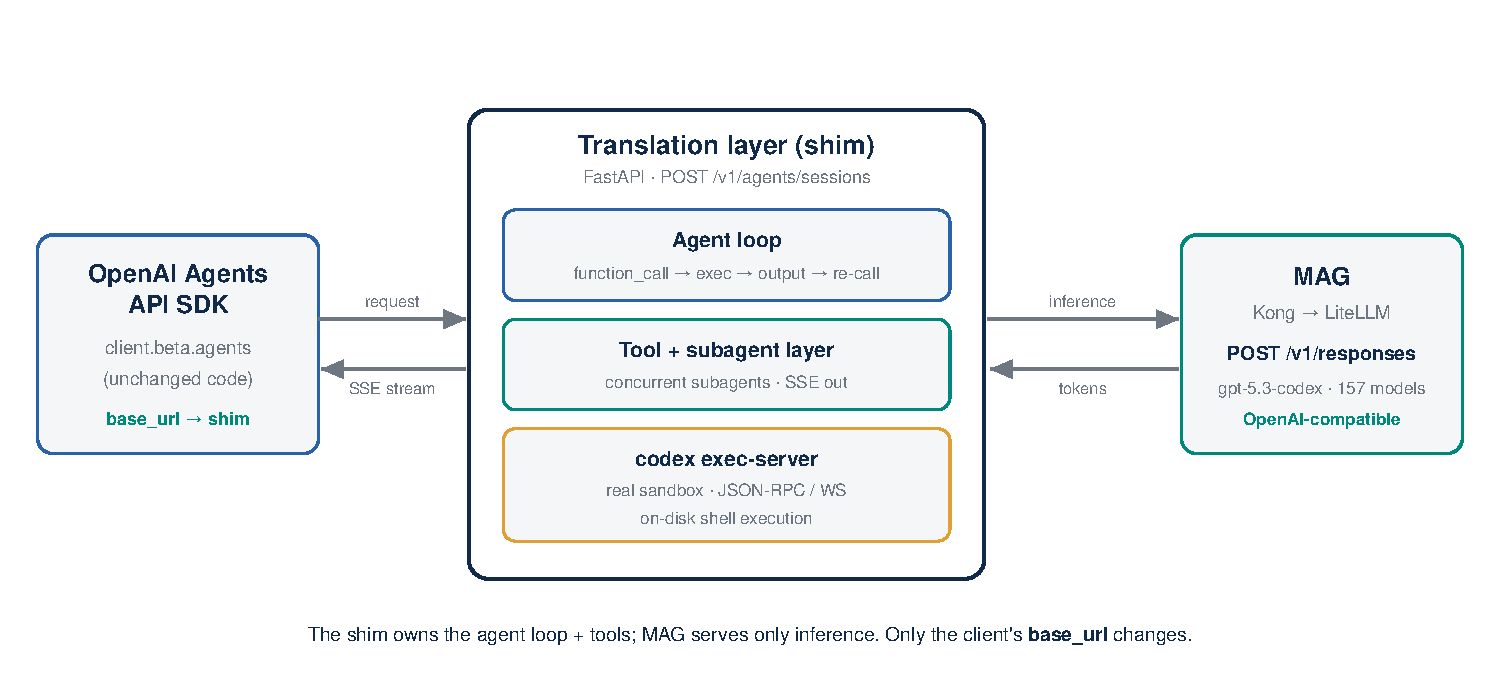
\includegraphics[width=0.96\textwidth,height=0.72\textheight,keepaspectratio]{architecture.pdf}
  \end{center}
\end{frame}

% ------------------------------------------------------------------ what's built
\begin{frame}{What's built and proven --- the full chain executes live}
  \begin{columns}[t, totalwidth=\textwidth]
    \begin{column}{0.5\textwidth}
      \begin{featbox}{accentteal}{\faCheckDouble\ Core --- tested and passing}
        \small
        \begin{itemize}
          \item[\faCheck] Agents API contract $\rightarrow$ loop over MAG \texttt{/v1/responses}
          \item[\faCheck] \texttt{function\_call} $\rightarrow$ exec $\rightarrow$ output $\rightarrow$ re-call
          \item[\faCheck] \textbf{Real sandbox} (\texttt{codex exec-server}), on-disk effects
          \item[\faCheck] \textbf{Concurrent subagents}, each its own sandbox
          \item[\faCheck] Queue-based SSE, clean event interleave
        \end{itemize}
      \end{featbox}
    \end{column}
    \begin{column}{0.04\textwidth}\end{column}
    \begin{column}{0.46\textwidth}
      \begin{featbox}{accentteal}{\faCheckDouble\ Shipped since --- all live-tested}
        \small
        \begin{itemize}
          \item[\faCheck] Native streaming passthrough
          \item[\faCheck] \texttt{/responses/compact} wiring
          \item[\faCheck] \texttt{apply\_patch} / \texttt{fs} tools
          \item[\faCheck] Sandbox-policy hardening
          \item[\faCheck] Exact event schema, auth, persist, cancel
          \item[\faCheck] \textbf{Local (stdio) MCP servers via exec-server}
        \end{itemize}
      \end{featbox}
    \end{column}
  \end{columns}
  \vspace{2pt}
  \begin{center}
    {\footnotesize\color{midgray}\textbf{5/5} live suites green vs MAG \,$\cdot$\, \textbf{24/24} SDK-model checks \,$\cdot$\, remaining items none blocked by MAG.}
  \end{center}
\end{frame}

% ------------------------------------------------------------------ the proof
\begin{frame}{The proof: OpenAI's own SDK examples run \emph{unchanged}}
  \small
  \begin{center}
  \renewcommand{\arraystretch}{1.3}
  \begin{tabular}{@{}l l l@{}}
    \toprule
    \textbf{Example (Rick Stevens' repo)} & \textbf{Exercises} & \textbf{Result} \\
    \midrule
    \texttt{01\_basic\_session.py} & SDK non-stream session & \textcolor{accentteal}{\faCheck\ exit 0} \\
    \texttt{03\_multi\_agent\_review.py} & streaming + multi-agent & \textcolor{accentteal}{\faCheck\ 2 subagents} \\
    \texttt{05\_raw\_curl.sh} & raw HTTP/SSE lifecycle & \textcolor{accentteal}{\faCheck\ full cycle} \\
    \bottomrule
  \end{tabular}
  \end{center}
  \vspace{8pt}
  \begin{calloutbox}[accentteal]
    \small\faKey\ The \textbf{only} change is
    \texttt{OPENAI\_BASE\_URL=http://127.0.0.1:8811/v1}. The example code is
    byte-for-byte upstream. Session objects + streaming events validated
    against real \texttt{openai==3.13.0} models --- \textbf{24/24}.
  \end{calloutbox}
\end{frame}

% ------------------------------------------------------------------ impl: loop
\begin{frame}{Inside the adapter: the server-side agent loop}
  \begin{columns}[t, totalwidth=\textwidth]
    \begin{column}{0.52\textwidth}
      \begin{featbox}{accentblue}{\faIcon{sync-alt}\ The per-turn loop}
        \small
        \setbeamertemplate{itemize items}[circle]
        \begin{enumerate}
          \item Client \texttt{POST /v1/agents/sessions} $\rightarrow$ shim opens SSE, emits \texttt{turn.in\_progress}
          \item Shim calls MAG \texttt{/v1/responses} (\texttt{stream:true}); forwards token deltas \emph{live}
          \item Model emits \texttt{function\_call} $\rightarrow$ dispatch to sandbox tool $\rightarrow$ feed output back $\rightarrow$ re-call MAG
          \item Repeat until a final message $\rightarrow$ \texttt{turn.completed}
        \end{enumerate}
      \end{featbox}
    \end{column}
    \begin{column}{0.04\textwidth}\end{column}
    \begin{column}{0.44\textwidth}
      \begin{featbox}{accentteal}{\faIcon{sitemap}\ Module map}
        \scriptsize
        \renewcommand{\arraystretch}{1.3}
        \begin{tabular}{@{}l l@{}}
          \texttt{mag\_agents\_shim.py} & loop, SSE, sessions, cancel \\
          \texttt{agents\_api\_models.py} & exact event/item builders \\
          \texttt{codex\_sandbox.py} & exec-server, fs, patch \\
          \texttt{mcp\_stdio.py} & MCP over exec-server \\
        \end{tabular}
      \end{featbox}
      \vspace{4pt}
      \begin{center}
        {\scriptsize\color{midgray}The loop OpenAI runs server-side ---
        re-served on top of MAG inference.}
      \end{center}
    \end{column}
  \end{columns}
\end{frame}

% ------------------------------------------------------------------ impl: details
\begin{frame}{Three details that made the translation faithful}
  \begin{columns}[t, totalwidth=\textwidth]
    \begin{column}{0.32\textwidth}
      \begin{featbox}{accentteal}{\faIcon{shield-alt}\ Real sandbox}
        \scriptsize
        Tools run in \texttt{codex exec-server}, launched \textbf{hardened}
        (\texttt{disk-write-cwd} + read-only elsewhere), each session its own
        workspace. A persistent-process \textbf{stdio bridge}
        (\texttt{process/start}$+$\texttt{process/write}) even drives local
        \textbf{MCP servers} in-sandbox.
      \end{featbox}
    \end{column}
    \begin{column}{0.02\textwidth}\end{column}
    \begin{column}{0.32\textwidth}
      \begin{featbox}{accentblue}{\faIcon{compress-alt}\ Compaction quirk}
        \scriptsize
        MAG \texttt{/responses/compact} \textbf{rejects its own} $>$64-char
        response IDs, so it can't chain by \texttt{previous\_response\_id}.
        Worked around via the \texttt{\{model,input\}} form; the non-input
        \texttt{compaction} item is cleaned back into reusable history.
      \end{featbox}
    \end{column}
    \begin{column}{0.02\textwidth}\end{column}
    \begin{column}{0.32\textwidth}
      \begin{featbox}{accentteal}{\faIcon{stream}\ Faithful wire}
        \scriptsize
        Streaming is a \textbf{live passthrough} of MAG deltas (not post-hoc
        chunking). A \textbf{cancel-race guard} aborts mid-tool, not just at
        turn boundaries. Every event/item validated against real
        \texttt{openai==3.13.0} --- \textbf{24/24}.
      \end{featbox}
    \end{column}
  \end{columns}
  \vspace{8pt}
  \begin{center}
    {\footnotesize\color{midgray}Each was reverse-engineered from MAG / the
    exec-server live, then locked down with a test.}
  \end{center}
\end{frame}

% ------------------------------------------------------------------ two paths
\begin{frame}{Two paths --- the decision hinges on where the 50B tokens live}
  \begin{columns}[t, totalwidth=\textwidth]
    \begin{column}{0.47\textwidth}
      \begin{featbox}{accentblue}{\faServer\ OpenAI-platform grant}
        \small Managed Agents API works \textbf{natively} --- but on
        \textbf{OpenAI's models}; MAG is not in the loop. (You may still
        self-host the \emph{sandbox} near your data.)
      \end{featbox}
    \end{column}
    \begin{column}{0.06\textwidth}\end{column}
    \begin{column}{0.47\textwidth}
      \begin{featbox}{accentteal}{\faDatabase\ AMSC / MAG allocation}
        \small Use the \textbf{self-hosted Codex harness} (or this adapter)
        pointed at MAG. The managed API cannot be used without the product
        change on the next slide.
      \end{featbox}
    \end{column}
  \end{columns}
  \vspace{12pt}
  \begin{center}
    {\color{midgray}For the 50B-token run \emph{now}: self-host against MAG ---
    \textbf{no OpenAI dependency}.}
  \end{center}
\end{frame}

% ------------------------------------------------------------------ the ask
\begin{frame}{The one ask to OpenAI --- and what already works today}
  \begin{calloutbox}[labnavy]
    \faBullhorn\ \textbf{Add a custom-model-provider / \texttt{base\_url} to the
    Agents API}, so the managed harness can route inference to an
    OpenAI-compatible endpoint (MAG) instead of OpenAI's hosted models.
  \end{calloutbox}
  \vspace{8pt}
  \small
  \begin{center}
  \renewcommand{\arraystretch}{1.25}
  \begin{tabular}{@{}l l@{}}
    \toprule
    \textbf{Need} & \textbf{Route} \\
    \midrule
    Agents on MAG, you control the client & Agents \emph{SDK} + \texttt{ModelProvider(base\_url)} --- no infra \\
    Existing \emph{managed-API} code on MAG & \textbf{this adapter}, until OpenAI ships the hook \\
    \bottomrule
  \end{tabular}
  \end{center}
  \vspace{6pt}
  \begin{center}
    {\footnotesize\color{midgray}The ask is \emph{only} for the managed Agents
    API. The SDK path needs no product change.}
  \end{center}
\end{frame}

% ------------------------------------------------------------------ scale-up
\begin{frame}{Before a 50B-token run: four items to close with AMSC}
  \begin{center}
  \begin{minipage}{0.9\textwidth}
    \setbeamertemplate{itemize items}[circle]
    \begin{itemize}
      \item[\faIcon{tachometer-alt}] \textbf{Per-key concurrency + TPM/RPM} --- agentic
        Codex is bursty; one agent opens dozens of concurrent requests.
      \item[\faIcon{exchange-alt}] Is \texttt{/v1/responses} \textbf{rate-limited
        differently} from \texttt{/v1/chat/completions}?
      \item[\faChartLine] \textbf{Sustained throughput headroom} for 50B tokens
        (tokens/sec; a batch / priority lane?).
      \item[\faReceipt] \textbf{Server-side usage accounting} to track burn
        against the allocation.
    \end{itemize}
  \end{minipage}
  \end{center}
  \vspace{6pt}
  \begin{center}
    {\footnotesize\color{midgray}MAG docs currently list no rate limits or quotas
    (``usage info coming soon'').}
  \end{center}
\end{frame}

% ------------------------------------------------------------------ recommendation
\begin{frame}{Recommendation}
  \begin{columns}[t, totalwidth=\textwidth]
    \begin{column}{0.5\textwidth}
      \begin{featbox}{accentteal}{\faRocket\ Ship now}
        \small Self-host the Codex harness (or this adapter) against MAG for the
        50B-token run. \textbf{No OpenAI dependency.}
      \end{featbox}
    \end{column}
    \begin{column}{0.04\textwidth}\end{column}
    \begin{column}{0.46\textwidth}
      \begin{featbox}{accentblue}{\faHandshake\ Press OpenAI}
        \small For managed-API portability, ask for the \texttt{base\_url} hook
        --- bring this repo as evidence the integration is straightforward.
      \end{featbox}
    \end{column}
  \end{columns}
  \vspace{14pt}
  \begin{center}
    \faGithub\ \textbf{Working proof:}\quad
    {\small\texttt{github.com/zhenghh04/amsc-mag-agents-api-adapter}}
  \end{center}
  \vspace{4pt}
  \begin{center}
    {\footnotesize\color{midgray}Public, secret-free; SDK examples reproduce with
    \texttt{bash scripts/run\_examples.sh}.}
  \end{center}
\end{frame}

% ------------------------------------------------------------------ getting started
\begin{frame}{Getting started: get a MAG token, then run}
  \begin{columns}[t, totalwidth=\textwidth]
    \begin{column}{0.5\textwidth}
      \begin{featbox}{accentblue}{\faKey\ 1 --- Get a MAG token (PAT)}
        \small
        \setbeamertemplate{itemize items}[circle]
        \begin{itemize}
          \item Log in at \texttt{portal-lite.genesis.\\american-science-cloud.org} (Ping Identity)
          \item Select your \textbf{Genesis Mission RFA} project $\rightarrow$ \textbf{switch}
          \item \textbf{Personal Access Tokens} $\rightarrow$ \textbf{Generate PAT} $\rightarrow$ copy once
        \end{itemize}
      \end{featbox}
      \vspace{4pt}
      \begin{calloutbox}[labnavy]
        \scriptsize\faInfoCircle\ Same PAT works for both wire APIs:\\
        OpenAI: \texttt{.../v1} \quad\textbullet\quad Anthropic: \texttt{.../} (root)
      \end{calloutbox}
    \end{column}
    \begin{column}{0.04\textwidth}\end{column}
    \begin{column}{0.46\textwidth}
      \begin{featbox}{accentteal}{\faTerminal\ 2 --- Configure \& run}
        \scriptsize
        \texttt{cp env.example .env}\\
        \texttt{\# set MAG\_API\_KEY = your PAT}\\[3pt]
        \texttt{\# sanity check:}\\
        \texttt{curl .../v1/models \textbackslash}\\
        \texttt{~~-H "Authorization: Bearer \$KEY"}\\[3pt]
        \texttt{bash scripts/run\_all.sh}\\
        \texttt{bash scripts/run\_examples.sh}
      \end{featbox}
      \vspace{4pt}
      \begin{center}
        {\scriptsize\color{midgray}Docs: \texttt{amsc-docs-d762d2.gitlab.io/}\\
        \texttt{model-access-gateway}}
      \end{center}
    \end{column}
  \end{columns}
\end{frame}

% beamer-slides house acknowledgement slide.
% Hard rule: for any deck about ALCF-supported work, this is the last content
% slide (before a "Thank you" / "Questions" slide, if you have one). Copy this
% text VERBATIM — do not paraphrase or shorten it.

\begin{frame}[plain]{Acknowledgement}
  \vfill
  \begin{center}
  \begin{minipage}{0.85\textwidth}
    \small
    This research used resources of the Argonne Leadership Computing
    Facility, a U.S.\ Department of Energy (DOE) Office of Science user
    facility at Argonne National Laboratory and is based on research
    supported by the U.S.\ DOE Office of Science-Advanced Scientific
    Computing Research Program, under Contract No.\ DE-AC02-06CH11357.
  \end{minipage}
  \end{center}
  \vfill
\end{frame}


% ------------------------------------------------------------------ thanks
\begin{frame}[plain]
  \vfill
  \begin{center}
    {\Huge\bfseries\color{labnavy}Thank you}\par
    \vspace{10pt}
    {\large\color{midgray}Questions?}\par
    \vspace{16pt}
    {\footnotesize\color{midgray}\faGithub\ github.com/zhenghh04/amsc-mag-agents-api-adapter
    \quad\textbullet\quad \faEnvelope\ \deckemail}
  \end{center}
  \vfill
\end{frame}

\end{document}
